\documentclass{article}
\usepackage[utf8]{inputenc}
% \usepackage{fontspec}
% \setmainfont{Times New Roman}

\usepackage{geometry}
\usepackage{natbib}
\usepackage{graphicx}

% 给文中的链接标识
\usepackage[colorlinks,linkcolor=red,anchorcolor=blue,citecolor=green]{hyperref}

% 设置页面边距
\geometry{a4paper,left=2cm,right=2cm,top=1cm,bottom=1cm}
% \geometry{a4paper,scale=0.8}

\begin{document}
	
	\title{Advances of Deep Learning}
	\author{James Smith}
	\date{May 2021}
	\maketitle
	
	\begin{abstract}
		This is a abstract of this article at the beginning of ths doucument
	\end{abstract}
	
	\section{Introduction}
	There is a theory which states that if ever anyone discovers exactly what the Universe is for and why it is here in Figure \ref{fig:universe} , it will instantly disappear and be replaced by something even more bizarre and inexplicable.\citep{adams1995hitchhiker}
	There is another theory which states that this has already happened.
	
	\begin{figure}[h!]
		\centering
		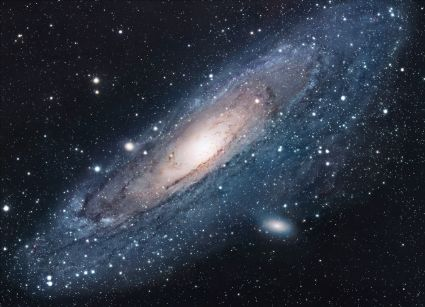
\includegraphics[scale=3]{img/universe}
		\caption{The Universe}
		\label{fig:universe}
	\end{figure}
	
	\section{Conclusion}
	``I always thought something was fundamentally wrong with the universe'' \citep{adams1995hitchhiker}
	
	
	\begin{itemize}
		\item This is test!
		\item Two!
	\end{itemize}
	
	\bibliographystyle{plain}
	\bibliography{references}
\end{document}
